\chapter{Snort and Security Onion}
\minitoc
\emph{In this chapter, a brief overview of Snort and its components will be provided. In the next chapter,  actual network penetration tests will take place and Snort will be monitored how well it picks up on those attacks.}

\section{What is Snort?}

Based on the different types of classifications introduced in the previous chapters, one could classify Snort as a ``Signature-based Network Intrusion Detection and Prevention System''.

Additionally, Snort is open-source and capable of performing real-time network traffic analysis, as well as packet logging on IP networks. It consists of two major parts: the detection engine and the rules that are used to describe traffic that has to be collected or blocked. Furthermore, there exist two types of rules: rules that are available to all users (the so-called ´´Community Rules) and private, proprietary (paid) rules that are developed by SourceFire, the company behind Snort \citep{SnortLicense}.

In this paper, I will make use of the freely available community rules. As one will notice, it will turn out that these rules are rather basic and need to be extende as well as additional rules have to be added in order to make Snort a viable IDS. This is allowed, since Snort uses the GPL license and we will make extensive use of this privilege to freely modify the rules.

As mentioned in the above paragraphs, Snort uses pre-defined rules to detect malicious activity on the network. One could compare it with the way antivirus programs work: any traffic that Snort picks up is matched against the database of rules and when a match has been found, an alert is raised.

\subsection{Preprocessors}

Preprocessors extend the functionality of Snort by examining packets or by modifying them so that Snort can properly interpret the packets. \citep{Preprocessor1}.

Some attacks cannot be detected by normal signatures (rules), so ``examine'' preprocessors detect suspicious behaviour. So one could say this type of preprocessor is used to detect non-signature-based attacks \citep{Preprocessor1}. 

The othe type of preprocessor is used to normalize traffic, so that Snort can match signatures in an accurate way.\\ \\
Preprocessor code is run before the detection engine is called. Additionally, each packet captured by Snort is cycled through every preprocessor, in order to discover even more attacks \citep{Preprocessor2}.

\subsection{PulledPork}

PulledPork (PP) is Perl script that will automatically download new Snort rules (signatures) in the background. Of course, one can always run PP directly at the command line to force the downloading of new rules \citep{PP}.

The downloaded rules are stored in a file called ``download.rules''.

\subsection{Barnyard2}

Barnyard2 is an interpreter for Snort binary output files. It is available under the GPL license and therefore, free to use \citep{Barnyard1}.

Barnyard2 allows Snort to write data to the disk in an efficient way. The parsing of binary data into different formats is handed over to a seperate process. Because Barnyard2 takes away some work, Snort will not miss any network traffic \citep{Barnyard2}.

\section{What is Security Onion?}

Security Onion is an Xubuntu-based Linux distribution that consists of packet-capturing programs, network - and host-based intrusion detection systems and various analysis tools \citep{SO1}.

\subsection{Packet capturing}

Packet capturing is accomplished by a program called ``netsniff-ng''. Via a network interface set to promiscious mode, netsniff-ng captures all the traffic the sensors (explained later) of Security Onion see and store as much of the information as possible. I.e., until the hard drive is full. Of course, Security Onion has a build-in mechanism to purge old data when the amount of data reaches a pre-defined level \citep{SO1}.

One could compare packet capturing with a video camera, that precisely sees and registers who, when and where was. The video camera is netsniff-ng and the persons walking around are the packets. All this is registered in a database.

Additionally, a video camera is also capable of registering of what people took with them. This is also the case with packet capturing: the payload of the packets can be examined as well as the destination address of the packets.

\subsection{NIDS and HIDS}

Network-based (NIDS) and host-based intrusion detection systems (HIDS) analyse the traffic that netsniff-ng captures and will log any malicious packets as well as sending alerts. Security Onion provides multiple IDS: two NIDS and one HIDS \citep{SO1}. \\
\textbf{NIDS}
\begin{itemize}
\item Signature-based NIDS: Snort or Suricata. In this paper, Snort will be used.
\item Anomaly-based NIDS: Bro IDS. The definition of anomaly-based IDSs has been covered in the previous chapters and since Snort will be used, we will not dive deeper into Bro.
\end{itemize}
\textbf{HIDS}
\begin{itemize}
\item OSSEC: an open-source HIDS for Windows, Linux and Mac OS X. Instead of monitoring an entire network, OSSEC monitores only one specific host on suspicious activity \citep{OSSEC}.
\end{itemize}

\subsection{Analyis tools}

With Snort / Suricata data and the packet capturing of netsniff-ng, there is a vast amount of data available for the analist. To help managing the alerts generated by Snort or Suricata, Security Onion comes with a handful of tools.

\begin{itemize}
\item Sguil: a network security analysis tool providing an intuitive GUI that provides access to realtime events and raw packet capturing data. The client is written in tcl/tk. In the client, one can view alerts of Snort, Bro, Suricata and OSSEC \citep{Sguil}.

The alerts are stored in a seperate MySQL database and this allows a user to query alerts by type, IP address or port, for example.

With Sguil, it is also possible to categorize alerts. This can be done either manually or automatically. The next chapter will provide more details of how this can be achieved \citep{Sguil}.

\item Squert: a web application that is used to view and query event data for the Sguil database. One could see it as a web interface for the Sguil database. It is neither ment to be a real-time interface, nor a replacement for Sguil, but more to bring additional visualization options to Sguil \citep{Squert}.

\item Snorby: a RoR (Ruby On Rails) web application that allows one to visualize Snort and Suricata alerts as well as perform queries on them. For example, listing the most active IDS signatures, most active sensors, \ldots. While all this can also be done with the Sguil database, Snorby offers a web interface instead of manually querying the Sguil database. In contrast to Sguil and Squert, Snorby uses his own, seperate database \citep{Snorby}.
\end{itemize}

\subsection{Deployment scenarios}

Security Onion is build on a client-server model. The client is called a ``sensor'', whereas the server is called, well... the ``server''.

Security Onion allows for the possibility to install the client and the server on seperate machines, but for this paper, a standalone version has been chosen. This means that the sensor and server run both on the same machine \citep{SO1}.

\section{Installation and configuration of Security Onion}

SecurityOnion has been installed as a virtual machine on VirtualBox for Windows hosts. Please note that a detailed explanation and visual representation of the test lab will be provided in the next chapter.

Security Onion requires two network interfaces: one management interface and one sniffing interface. In VirtualBox, the sniffing interface will be set up using promiscious mode as illustrated in the following screenshots.

\clearpage

\begin{figure}[h!]
    \centering
    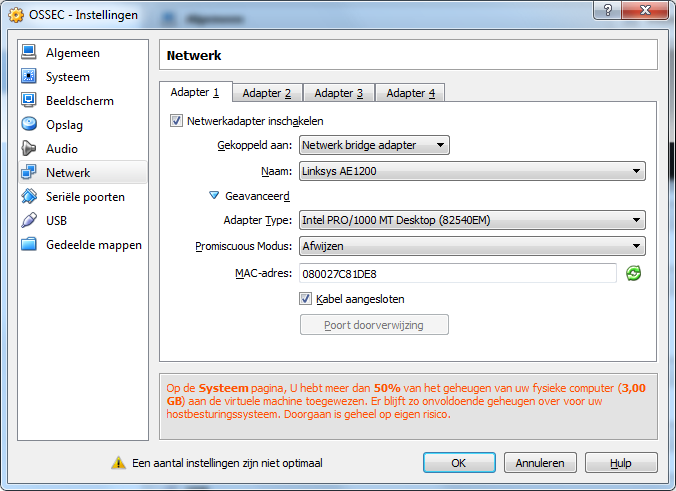
\includegraphics[width=0.75\textwidth]{VM_1.png}
    \caption{Configuration of the network settings in VirtualBox. The wireless network adapter is chosen as the management interface. In Security Onion, it will be listed as ``eth0''.}
\end{figure}

\begin{figure}[h!]
    \centering
    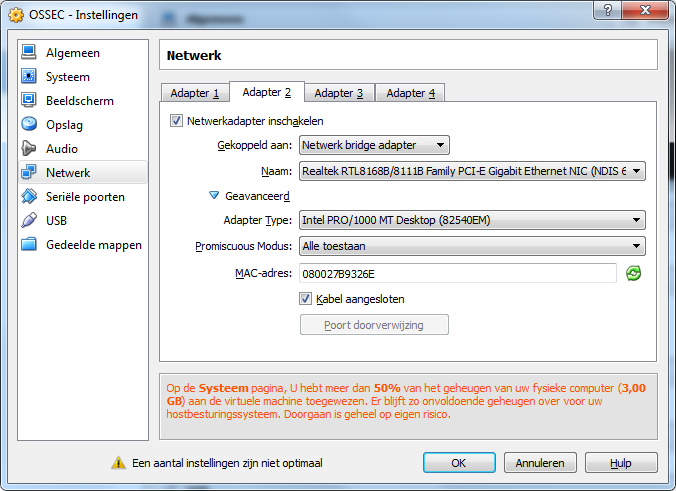
\includegraphics[width=0.75\textwidth]{VM_2.png}
    \caption{Configuration of the network settings in VirtualBox. The LAN adapter is chosen as the monitoring / sniffing interface. This will be ``eth1'' in Security Onion. As one can see, promiscious mode is set on this interface.}
\end{figure}

After the VirtualBox configuration has completed, the installation of Security Onion can start. The iso-file of Security Onion is freely available as download. Once downloaded, the iso-file can be mounted in VirtualBox and the VM can be started. \\ \\
When SO (Security Onion) has been installed (the installation is not covered in this paper as there exist various websites that cover the installation of SO.) Instead, only the configuration is explained in the following sections. \\ \\
When booting SO, a login and password have to be provided after which the user is authenticated and logged in. Next, SO has to be set up in order to use it with the current network.

\begin{figure}[h]
    \centering
    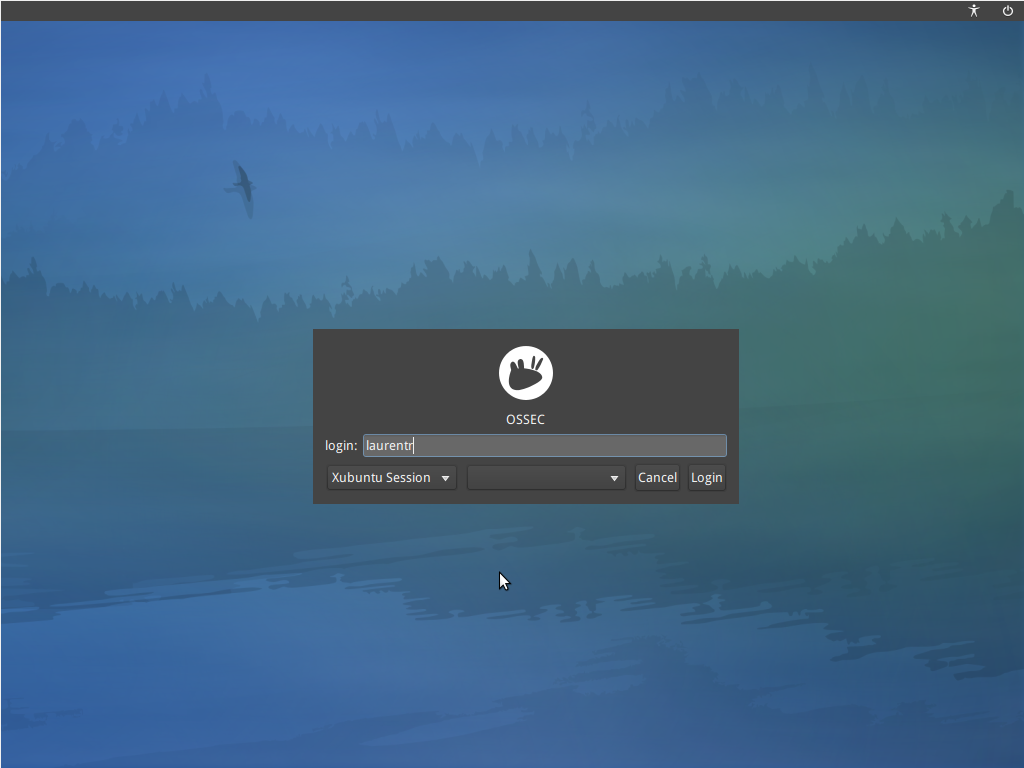
\includegraphics[width=0.95\textwidth]{VM_3.png}
    \caption{Login screen of Security Onion}
\end{figure}

Once SO is installed, the process of setting up SO can be started. This is done by clicking on ``Setup''.
\begin{figure}[h]
    \centering
    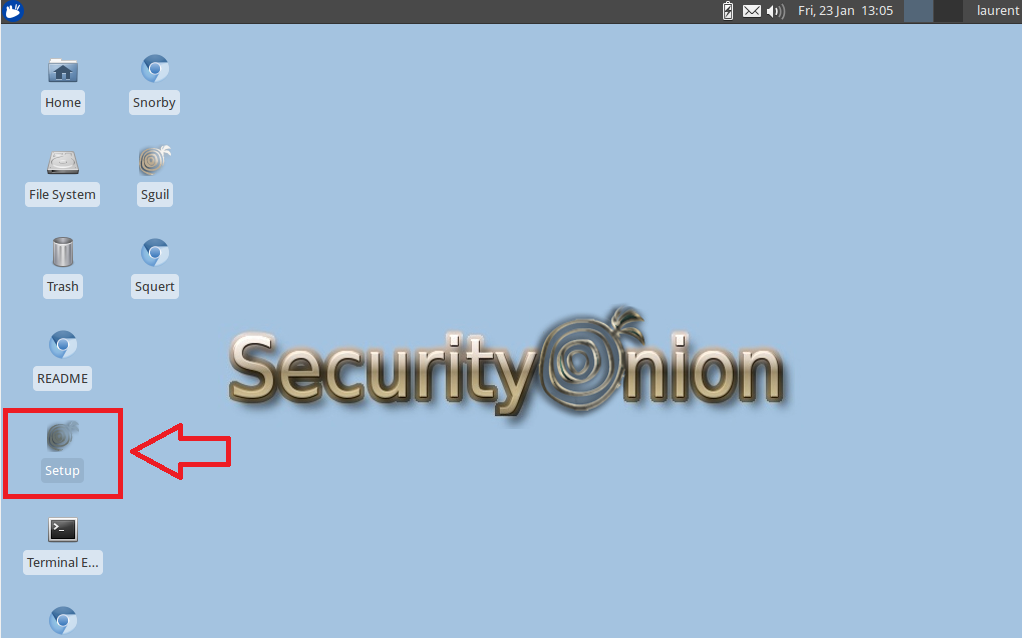
\includegraphics[width=0.95\textwidth]{VM_4.png}
    \caption{Begin the setup of SO by clicking on ``Setup''.}
\end{figure}

\begin{figure}[h]
    \centering
    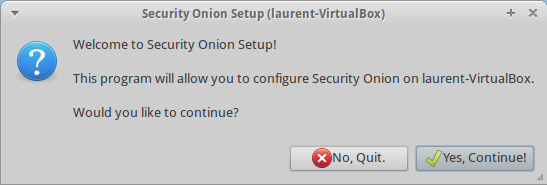
\includegraphics[width=0.85\textwidth]{VM_5.png}
    \caption{Obviously, we want to continue.}
\end{figure}
\clearpage
Next, the management interface has to be chosen. In our case, this is eth0, the wireless network adapter. The management interface is the normal interface that is used to communicate with the network. I.e., not the promiscious / sniffing interface.
\begin{figure}[h]
    \centering
    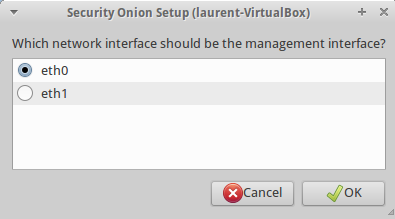
\includegraphics{VM_6.png}
    \caption{As previously mentioned, the wireless LAN adapter will be used as the management interface (eth0).}
\end{figure}

After having chosen the management interface, SO asks whether DHCP or static IP addressing has to be used. We opt for DHCP since we only use SO for testing purposes.
\begin{figure}[h]
    \centering
    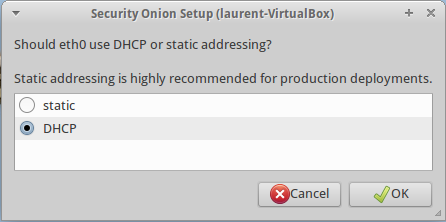
\includegraphics{VM_7.png}
    \caption{Since SO will only be used for testing purposes, DHCP can and will be chosen over a static IP.}
\end{figure}
\clearpage
As the management interface is set up, the sniffing interface can be configured. This is done in the next step. Our sniffing interface will be eth1 - the wired ethernet adapter. \\ \\
\begin{figure}[h]
    \centering
    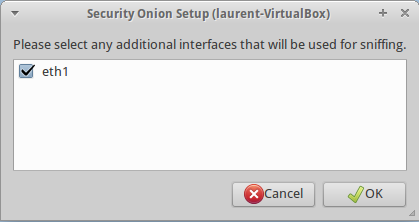
\includegraphics{VM_8.png}
    \caption{As previously mentioned, the wired LAN adapter will be used as the sniffing / monitoring interface (eth1).}
\end{figure}

Next, SO asks whether or not the new configuration can be made persistent. Obviously, we choose ``yes'' and the system is rebooted.
\begin{figure}[h!]
    \centering
  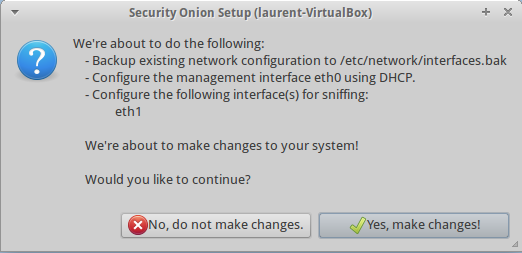
\includegraphics[width=0.65\textwidth]{VM_9.png}
  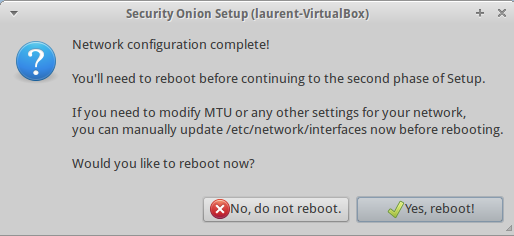
\includegraphics[width=0.65\textwidth]{VM_10.png}
    \caption{Configuration of the network interfaces has been completed. Time to reboot the system!}
\end{figure}
\clearpage
When the system has been rebooted, setup is entered again. SO will detect that the network interface have been configured and will proceed to the next phase of the configuration process: the configuration of Snort and Sguil. \\ \\
There exist two possibilities for the next phase. Either one choses to proceed with the basic, quick setup or one choses to proceed using the advanced setup. These are the differences: \\ \\
\textbf{Quick setup will}
\begin{itemize}
\item Configure SO to use Snort.
\item Monitor all network interfaces.
\item Enable Sguil, Squert and Snorby.
\end{itemize}
\textbf{Advanced setup will}
\begin{itemize}
\item Install either a Sguil server, Sguil sensor, or both.
\item Use either Snort or Suricata.
\item Provide the option to select an IDS ruleset.
\item Provide the choice of which network interface has to be configured.
\end{itemize}
We will opt for advanced setup. \\
\begin{figure}[h]
    \centering
    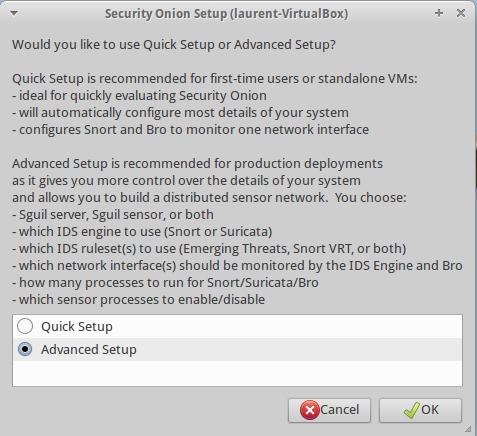
\includegraphics[width=0.70\textwidth]{VM_11.png}
    \caption{Since advanced setup offers more configuration options, this setup mode is chosen.}
\end{figure}

In our setup, the server and sensor will be installed on the same machine, so standalone configuration is chosen.
\begin{figure}[h]
    \centering
    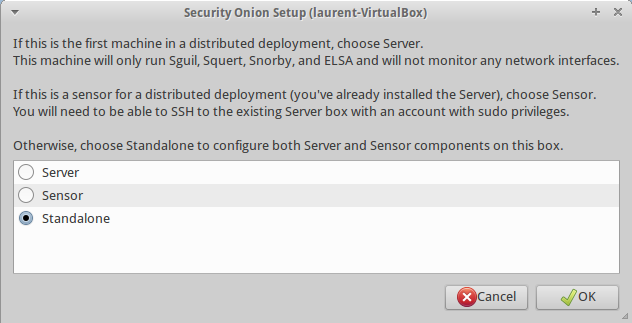
\includegraphics[width=0.90\textwidth]{VM_12.png}
    \caption{Since our test lab is small, a standalone setup is sufficient.}
\end{figure}
\clearpage
Next, a username, email address and password need to be chosen for logging in into Sguil, Squert and Snorby.
\begin{figure}[h]
    \centering
    	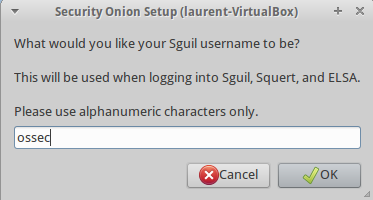
\includegraphics{VM_13.png}
	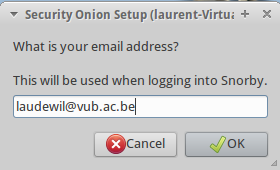
\includegraphics{VM_14.png}
 	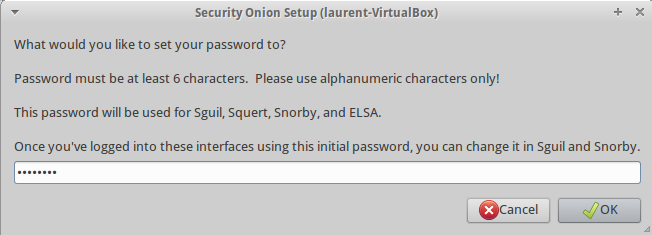
\includegraphics[width=0.85\textwidth]{VM_15.png}
    \caption{Selecting a username, email address and password respectively.}
\end{figure}

\clearpage
As previously mentioned, the Snort alerts are kept in the Sguil database. But of course, in a huge and noisy network, the tables can fill quickly with data. Therefore, Sguil offers the possibility to purge old data. In the next step, one has to select after how many days data has to be purged.
\begin{figure}[h]
    \centering
    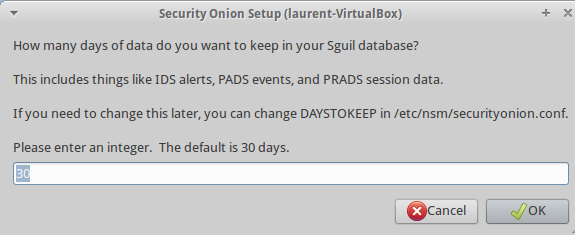
\includegraphics[width=0.85\textwidth]{VM_16.png}
    \caption{The number of days data has to be kept in the Sguil database.}
\end{figure}

In the next, important step, SO offers the choice of IDS. We will opt for Snort.
\begin{figure}[h]
    \centering
    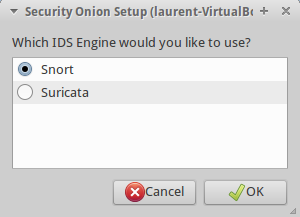
\includegraphics{VM_17.png}
    \caption{Chosing between Snort and Suricata}
\end{figure}

\clearpage
Next, SO offers the choice of ruleset. Since I use the community rules, ``Emerging Threats GPL'' is the logical choice.
\begin{figure}[h]
    \centering
    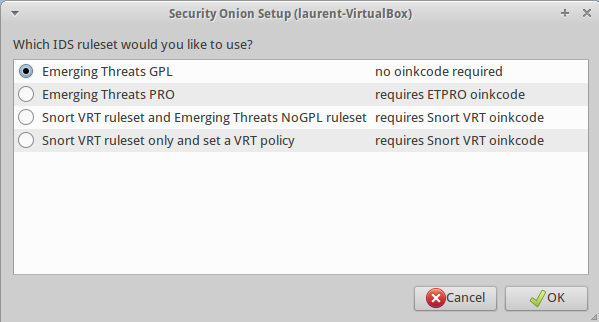
\includegraphics[width=0.85\textwidth]{VM_18.png}
    \caption{Emerging Threats GPL ruleset is the logical, non-paid choice.}
\end{figure}

Once again, the monitoring / sniffing interface has to be selected.
\begin{figure}[h]
    \centering
    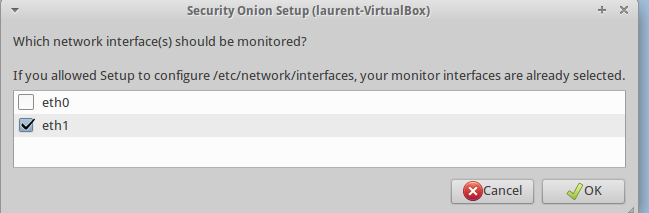
\includegraphics[width=0.85\textwidth]{VM_19.png}
    \caption{As selected before, the sniffing interface is eth1, the wired LAN interface.}
\end{figure}

\clearpage
Then, since we have multiple CPU cores available, we are presented with the option to select how many CPU cores we want to use with Snort. Since the physical machine has a dual-core processor, two instances (processes) of Snort will run on the system.
\begin{figure}[h]
    \centering
    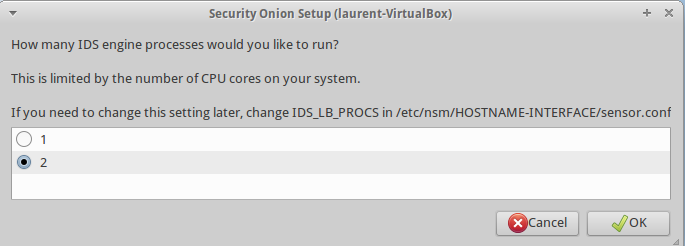
\includegraphics[width=0.85\textwidth]{VM_20.png}
    \caption{Since we have a dual-core processor available, two instances of Snort wil run on the system.}
\end{figure}

Eventually, with everything set and done, Security Onion can make the changes persistent after which the system has to be rebooted.
\begin{figure}[h]
    \centering
    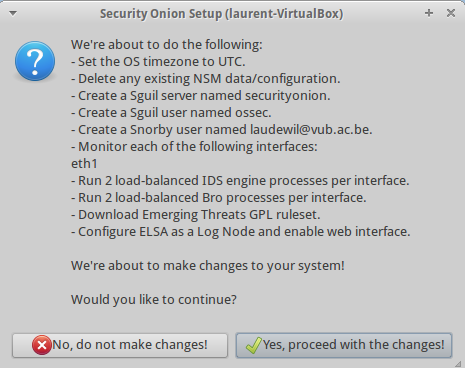
\includegraphics[width=0.55\textwidth]{VM_21.png}
    \caption{Apply the changes!}
\end{figure}

\clearpage
With Security Onion (and Snort and Sguil) installed and configured, we can start using it. Of course, in order to be sure whether Snort indeed picks up all the traffic that flows through the network, we must first test it.

This can be done by running Snort in test mode which yields following output. For this, I logged in into Security Onion using an SSH session.

\begin{figure}[h]
    \centering
    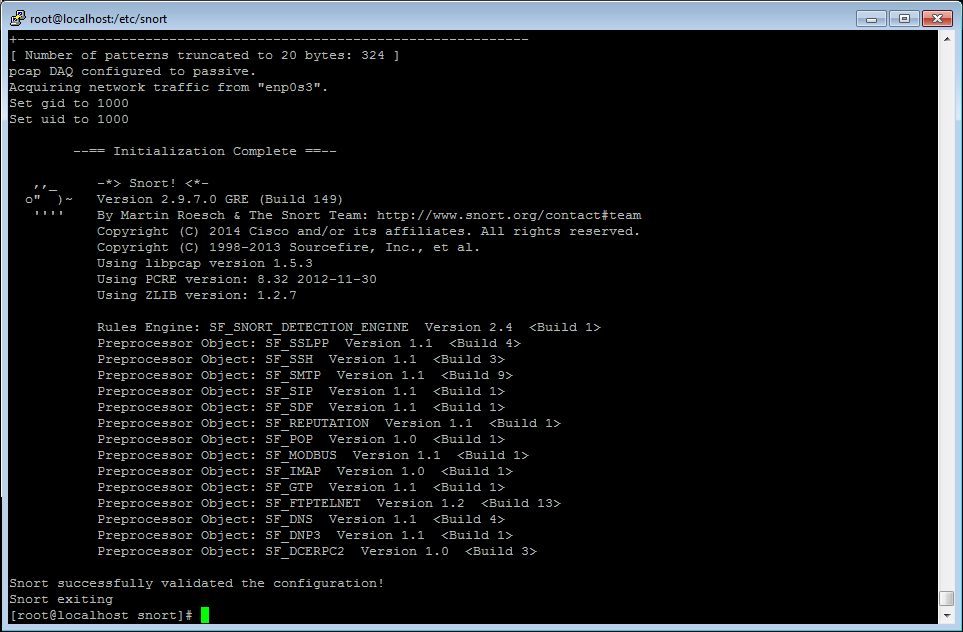
\includegraphics[width=0.55\textwidth]{Snort.jpg}
    \caption{Testing if Snort works correctly.}
\end{figure}

Now that everything has been installed correctly and the working of Snort has been verified, we can begin with penetration testing our network. This is the subject of the next chapter.